\chapter{Statistics}
\label{app:statistics}

\begin{section}{Profile likelihood}


This section presents an introduction to the profile likelihood method
(used for the statistical results of this thesis) with a concrete toy example.
The frequentist toy example consists of one signal, one background, and one shape-based
nuisance parameter. Complete details of the method are in Reference~\cite{STAT:Cowan2010js}.


\begin{subsection}{Terminology}

Bayes' theorem can be stated in a more applicable way as
\begin{equation}
p(k|D) = \frac{p(D|k)p(k)}{p(D)}
\end{equation}
where $p(A|B)$ is the (conditional) probability of A given B.
Here, $k$ represents a model, which consists of a set of parameters 
(parameters of interest, as well as annoying/nuisance parameters). 
Typically, the single parameter of interest is a signal ``strength'' $\mu$
    (how much signal is there actually, compared to what is nominally in the simulation -- $\mu = \mu_\mathrm{obs}/\mu_\mathrm{SM}$), 
 and a set of (many) nuisance parameters technically specified
as a vector $\vec{\theta}$, but could be just $\theta$. The posterior probability 
distribution function (pdf), $p(k|D)$ is the distribution of parameters given the observed
data D. The \textbf{likelihood} $p(D|k)$ gives the likelihood of getting some data $D$
given a particular model encoded in $k$. $p(k)$ is a prior distribution of models, often
taken to be ``flat'' in $\mu$. Lastly, the overall constant $p(D)$ is ignorable when dealing
with differences in likelihoods.

Analysis observables are typically binned into many regions, and compared with an observed count (data).
Integral data event counts (N) obey Poisson statistics, where $\lambda$ governs the underlying
rate of a process: $p(N|\lambda) = e^{-\lambda}\frac{\lambda^N}{N!}$ .
(Although, when statistics are large, Gaussian approximations can be made in order to simplify computations.)
For independent bins, the likelihood is a product over each of the bins.

This sets the stage for the toy example, which clarifies the meaning of the word \textbf{profile}.



\end{subsection}

\begin{subsection}{Toy example}

Figure~\ref{fig:toystat:njets} shows a toy distribution of jet multiplicity
for background, signal, and data. The background component also contains a
systematic uncertainty band corresponding to a shape nuisance parameter.
This shape nuisance parameter prefers to increase yields at higher number of jets.

\begin{figure}[!htb]
    \centering
    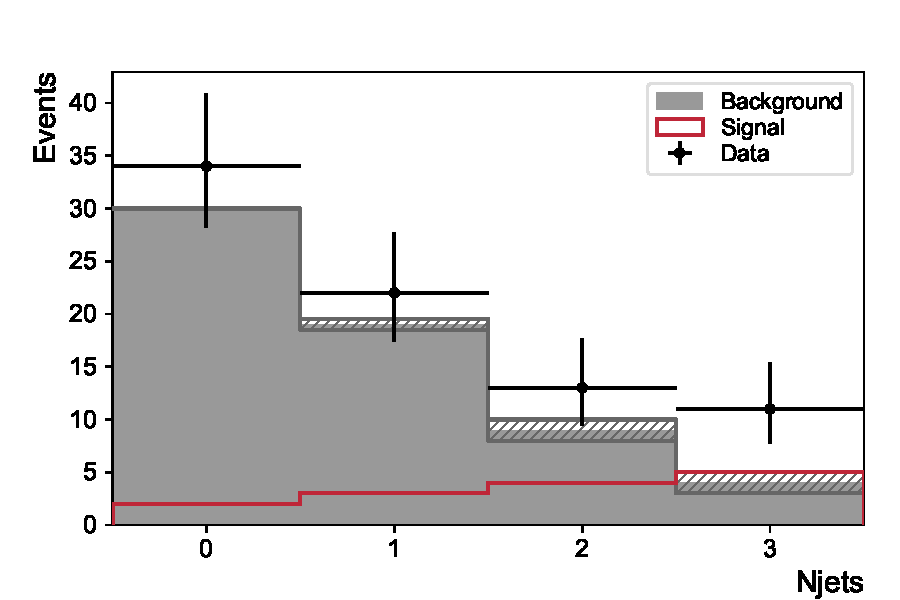
\includegraphics[width=0.48\linewidth]{figs/toy_statistics/njets.pdf}
    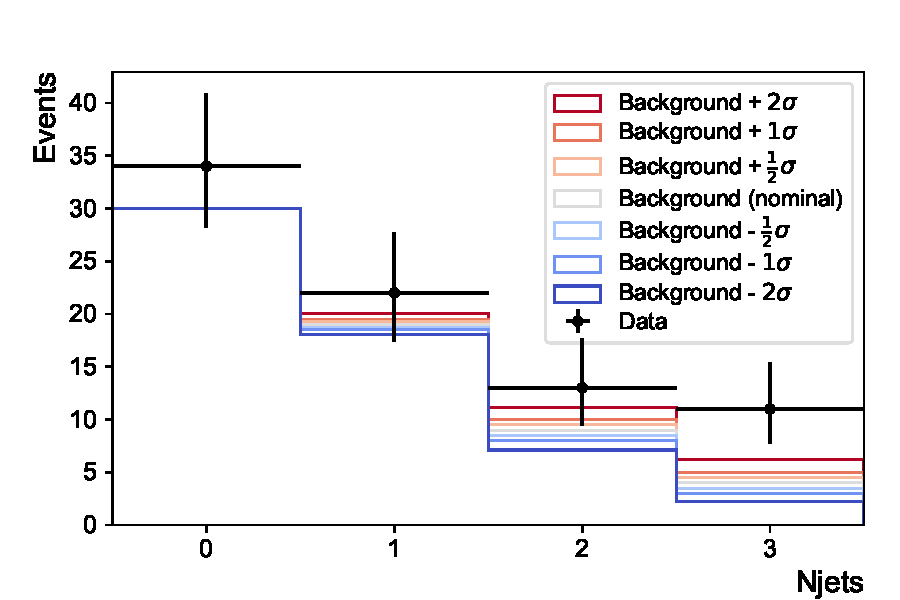
\includegraphics[width=0.48\linewidth]{figs/toy_statistics/backgroundvariations.pdf}
    \caption{
Toy distribution (left) and single shape nuisance variation on background component (right)
    }
    \label{fig:toystat:njets}
\end{figure}
    
As an intermediate goal to most statistical results/interpretations of the data,
we want to compute the likelihood which will be a 2D function of the
signal strength $\mu$ and the value of the systematic variation
$\theta$. $\theta=0$ will give the normal background yields, while
$\theta=-1$ and $\theta=1$ will give the $1\sigma$ down and up
variations, respectively. From above, $\theta=1$ will absorb
 the signal, as it increases the background yield at high number of
jets.

The likelihood function is the binned probability to get the data from a
$b$ (background-only) or $s+b$ (background and signal) poisson distribution, 
accounting for the probability of nuisances $\theta$ with the pdf $p(\theta)$:
\begin{equation}
\mathcal{L}(\mathrm{data}|\mu,\theta)=\prod_{j\in\mathrm{bins}}
\frac{(\mu s_j + b_j)^{n_j}}{n_j!}
e^{-(\mu s_j + b_j)}
p(\theta)
\end{equation}
 here $n_j$ represents the data count in bin $j$, $b_j$ the
background count, and $s_j$ the signal count. Technically, $b_j$ is
a function of $\theta$; that is, $b_j(\theta)$ depends on the value
of the systematic variation where $b_j(0)$ is the nominal background
yield.

The goal is find maxima in the likelihood scan. However, numbers can get very
large given the factorial and the exponential. Since the $\ln$
function is monotonically increasing, to make things numerically
tractable and simpler, we take the (negative) log
since minimization problems are easier than maximization. 
\begin{equation}
-\ln\mathcal{L}=-\sum_{j=0}^{3}\left[
n_j \ln(\mu s_j + b_j) - \ln(n_j!) - (\mu s_j + b_j) + \ln(p(\theta))
\right]
\end{equation}


Even though it won't matter in the end (since we ultimately care about
relative differences in the likelihood) note that $\ln(n_j!)$ is just
$\sum_{i=0}^{3}\ln(i)$ and it is independent of $\mu$ and
$\theta$, so it can usually be pre-computed.

We can then calculate likelihood values over the $\mu$-$\theta$ plane. 
Figure~\ref{fig:toystat:2dlikelihood} shows this two dimensional
likelihood scan as a function of $\theta$ and $\mu$, with contours overlaid,
as well as the global maximum log likelihood (the
minimum \emph{negative} log likelihood).
The plot also shows the maximum likelihood as a function of $\mu$
with a red line. Equivalently, this gives the nuisance parameter value that
maximizes the likelihood for a fixed $\mu$.

\begin{figure}[!htb]
    \centering
    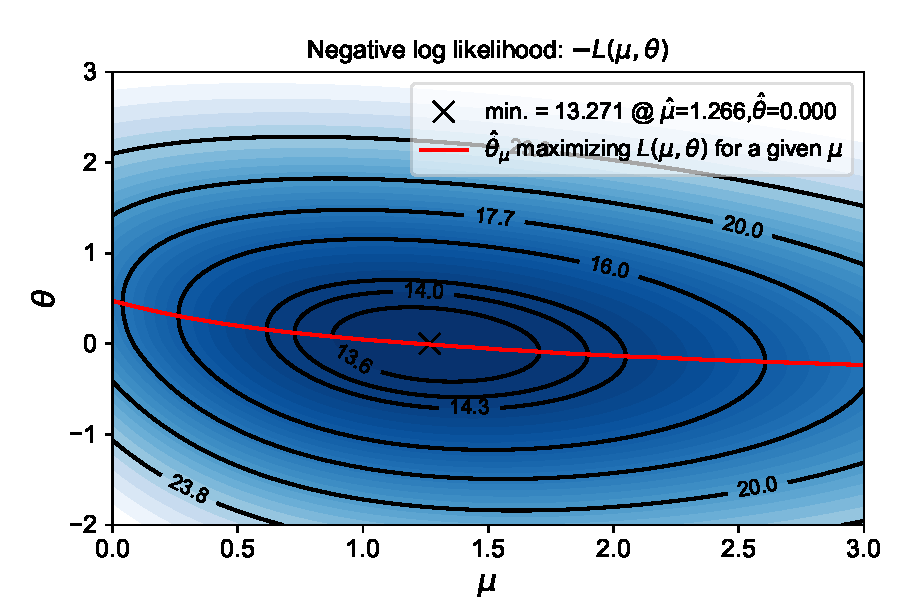
\includegraphics[width=0.80\linewidth]{figs/toy_statistics/likelihood_theta_vs_mu.pdf}
    \caption{
Two dimensional likelihood scan as a function of $\theta$ and $\mu$. The red line
shows the maximum likelihood for a given $\mu$.
    }
    \label{fig:toystat:2dlikelihood}
\end{figure}
    
From the two dimensional scan, we see the maximum global likelihood 
occurs when the signal strength parameter
$\mu$ is 1.27. This roughly makes sense given the histogram templates which had
5 signal, 4 background, and 11 observed events in the last bin.
This bin dominates the result due to the strong signal presence.
With the fitted signal strength, $5\times1.27 + 4 \approx 11$.

For lower values of $\mu$, the best likelihood values occur
for increasing $\theta$. This can be understood as a compensatory effect: when
signal yields decrease, in order to have background+signal match data,
we need to ``borrow'' some yields from the background nuisance, which
pulls up yields at higher number of jets. Of course, there is a likelihood penalty
to this due to the $p(\theta)$ term.

Figure~\ref{fig:toystat:theta} shows two curves of
$-\ln\mathcal{L}(\mu,\theta)$ for two
slices of the scan ($\mu=\hat{\mu}$, and $\mu=0$).

\begin{figure}[!htb]
    \centering
    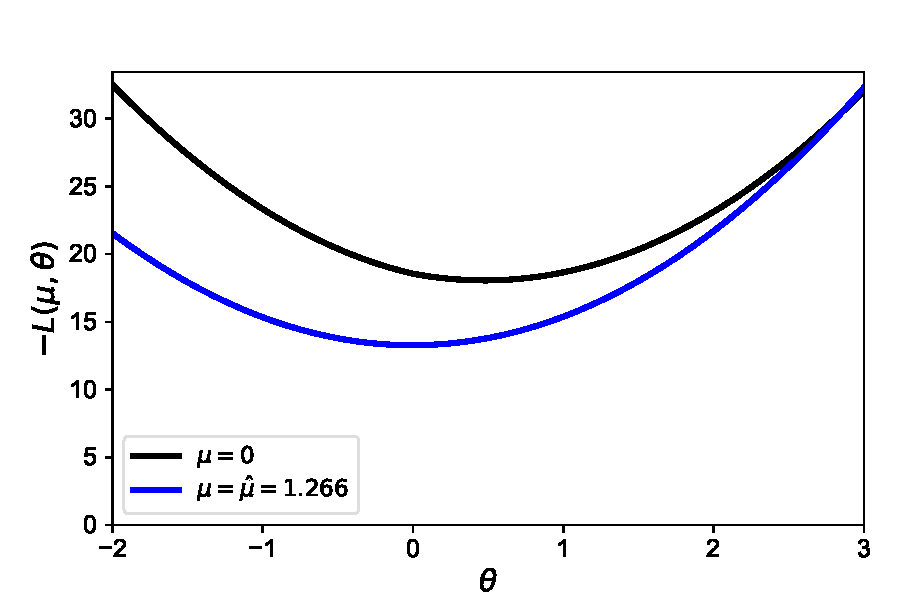
\includegraphics[width=0.80\linewidth]{figs/toy_statistics/likelihood_vs_theta.pdf}
    \caption{
Negative log likelihood as a function of $\theta$ for $\mu$ fixed to 0 and $\hat{\mu}$
    }
    \label{fig:toystat:theta}
\end{figure}

Let's define the LHC profiled test statistic $q_\mu$ as 
\begin{equation}\label{eq:qmu}
q_\mu = q(\mu) = -2\ln\frac{\mathcal{L}(\mu,\hat{\theta}_\mu)}{\mathcal{L}(\hat{\mu},\hat{\theta})}
\end{equation}
 where $\hat{\theta}_\mu$ is the $\theta$ that maximizes
$\mathcal{L}$ for a particular $\mu$. The pair $\hat{\mu}$ and
$\hat{\theta}$ are the ones that globally maximize the likelihood.
Thus, the denominator is a single number (the global extremum of the
2-dimensional likelihood scan). The numerator is a 1-dimensional function
which gives the maximum likelihood as a function of $\mu$. We have
``profiled out'' the nuisance parameter $\theta$. Bear in mind the
additional minus sign gymnastics we must do when switching between log
likelihood and negative log likelihood: 
\begin{equation}
q_\mu = 2\left[\mathrm{NLL}(\mu,\hat{\theta}_\mu) - \mathrm{NLL}(\hat{\mu},\hat{\theta})\right]
\end{equation}
 Or, $q_\mu$ is calculated as twice the difference of the negative log likelihood values
along the red curve from the two dimensional scan, and the global minimum negative log likelihood
from the same scan. Figure~\ref{fig:toystat:qmu} shows a plot of $q_\mu = q(\mu)$

\begin{figure}[!htb]
    \centering
    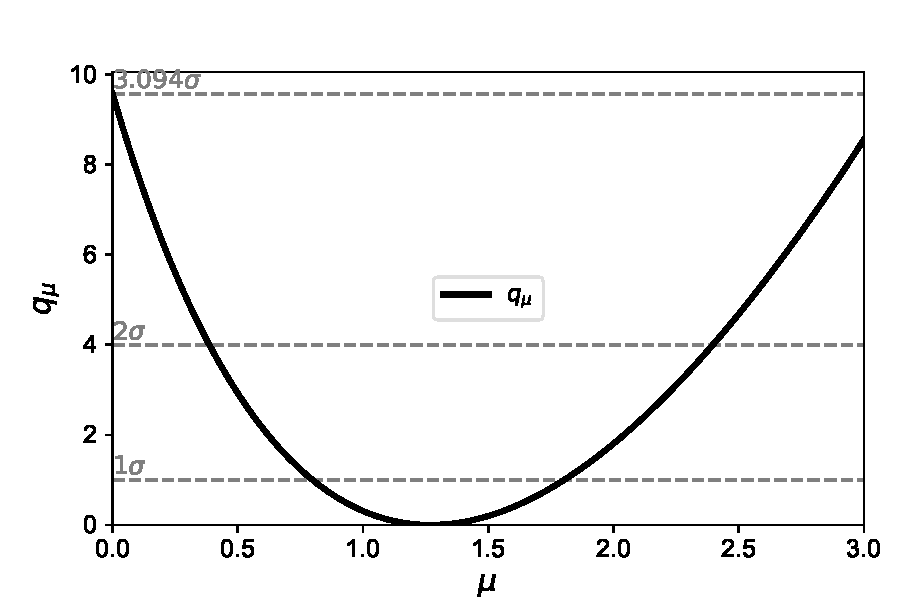
\includegraphics[width=0.80\linewidth]{figs/toy_statistics/qmu_vs_mu.pdf}
    \caption{
LHC test statistic as a function of $\mu$
    }
    \label{fig:toystat:qmu}
\end{figure}

Before proceeding, we now work with the asymptotic approximation in the case of large
background. That is, the test statistic $q_\mu$ with data containing signal strength $\mu'$
follows a Gaussian distribution 
\begin{equation}
    q_\mu = \frac{(\mu-\hat{\mu})^2}{\sigma^2} + \mathcal{O}(1/\sqrt{N})
\end{equation}
where $\hat{\mu}\sim \mathcal{N}(\mu',\sigma)$, $N$ is the sample size,
and $\sigma$ is the standard deviation of $\hat{\mu}$ which is extracted
from the covariance matrix of nuisances $\theta$. Ultimately, one finds that
with this approximation, the test statistic follows a noncentral chi-square distribution
for one degree of freedom. See the continuing discussion in Ref.~\cite{STAT:Cowan2010js}. 
This is exploited for huge computational gains, especially for SUSY scans which consist
of hundreds to a few thousand mass points (number of signal hypotheses to test with the data 
and background predictions).

Returning to the curve in Figure~\ref{fig:toystat:qmu}, we can identify the significance of the data from
one point. That is, how statistically significant would it be if just
the background (null hypothesis) fluctuated to look like background+signal: 
\begin{equation}
Z_\text{obs} = \sqrt{q_0}
\end{equation}
 And more generally, we can compute 1$\sigma$, 2$\sigma$,
3$\sigma$, etc. confidence bands on the fitted value of $\hat\mu$ by
drawing lines at $q_\mu=1,4,9,...$ . Why these values in particular? We turn to a
normal distribution with a pdf of
\begin{equation}
f(x|\mu,\sigma)=\frac{1}{\sqrt{2\pi\sigma^2}}e^{-\frac{(x-\mu)^2}{2\sigma^2}}
\end{equation}
Identifying this as a likelihood pdf and ignoring all constant/offset
terms independent of $\sigma$ and $\mu$, then 
\begin{equation}
q_\mu = -2\ln(f) = 2\frac{(x-\mu)^2}{2\sigma^2}
\end{equation}
 We want $x\rightarrow \mu+k\cdot\sigma$ and $k$ is
1,2,3,\ldots{}, so 
\begin{equation}
q_\mu \rightarrow \frac{(k\sigma)^2}{\sigma^2}=k^2
\end{equation}

In this toy example, based on Figure~\ref{fig:toystat:qmu}, the observed significance of the result is $3.09\sigma$
and the fitted signal strength, $\mu$, is approximately $1.3^{+0.4}_{-0.5}$.
For ``expected'' quantities, one can consider the \textbf{asimov} dataset, which is constructed
with background (or signal+background) expectation, incorporating fluctuations due to statistics as well
as systematics encoded by the nuisance parameters. This is done to understand analysis results, for example,
without looking at the real data.

\end{subsection}

\begin{subsection}{Upper limits}

For the purposes of setting upper limits on signal strengths, 
a modified version of Equation~\ref{eq:qmu} is used as the 
test statistic:

\begin{equation}
q_\mu = q(\mu) = -2\ln\frac{\mathcal{L}(\mu,\hat{\theta}_\mu)}{\mathcal{L}(\hat{\mu},\hat{\theta})}
\qquad \text{if}~\hat{\mu}\leq\mu\qquad \text{else}\qquad 0
\end{equation}

This is done so that data where $\hat{\mu}>\mu$ isn't penalized
for representing poorer compatibility with $\mu$ from actual data.
Armed with this modified test statistic,
to set upper limits with the 
\CLs method~\cite{STAT:Junk1999kv,STAT:Read2002hq,STAT:ATLPHYSPUB2011011,STAT:Cowan2010js},
we find
\begin{equation}
\mathrm{CL}_s(\mu) 
= \frac{\mathrm{CL}_{s+b}}{\mathrm{CL}_{b}}
= \frac{p(q_\mu \geq q_\mu^\text{obs} | \mu s + b)}{p(q_\mu \geq q_\mu^\text{obs} | b)}
= \frac{\text{R}}{1-\text{L}}
\end{equation}
and scan the quantity over $\mu$ until $\mathrm{CL}_s = 5\%$.
The last equality allows the equation to be identified schematically
with Figure~\ref{fig:ulschematic}
\begin{figure}[!htb]
    \centering
    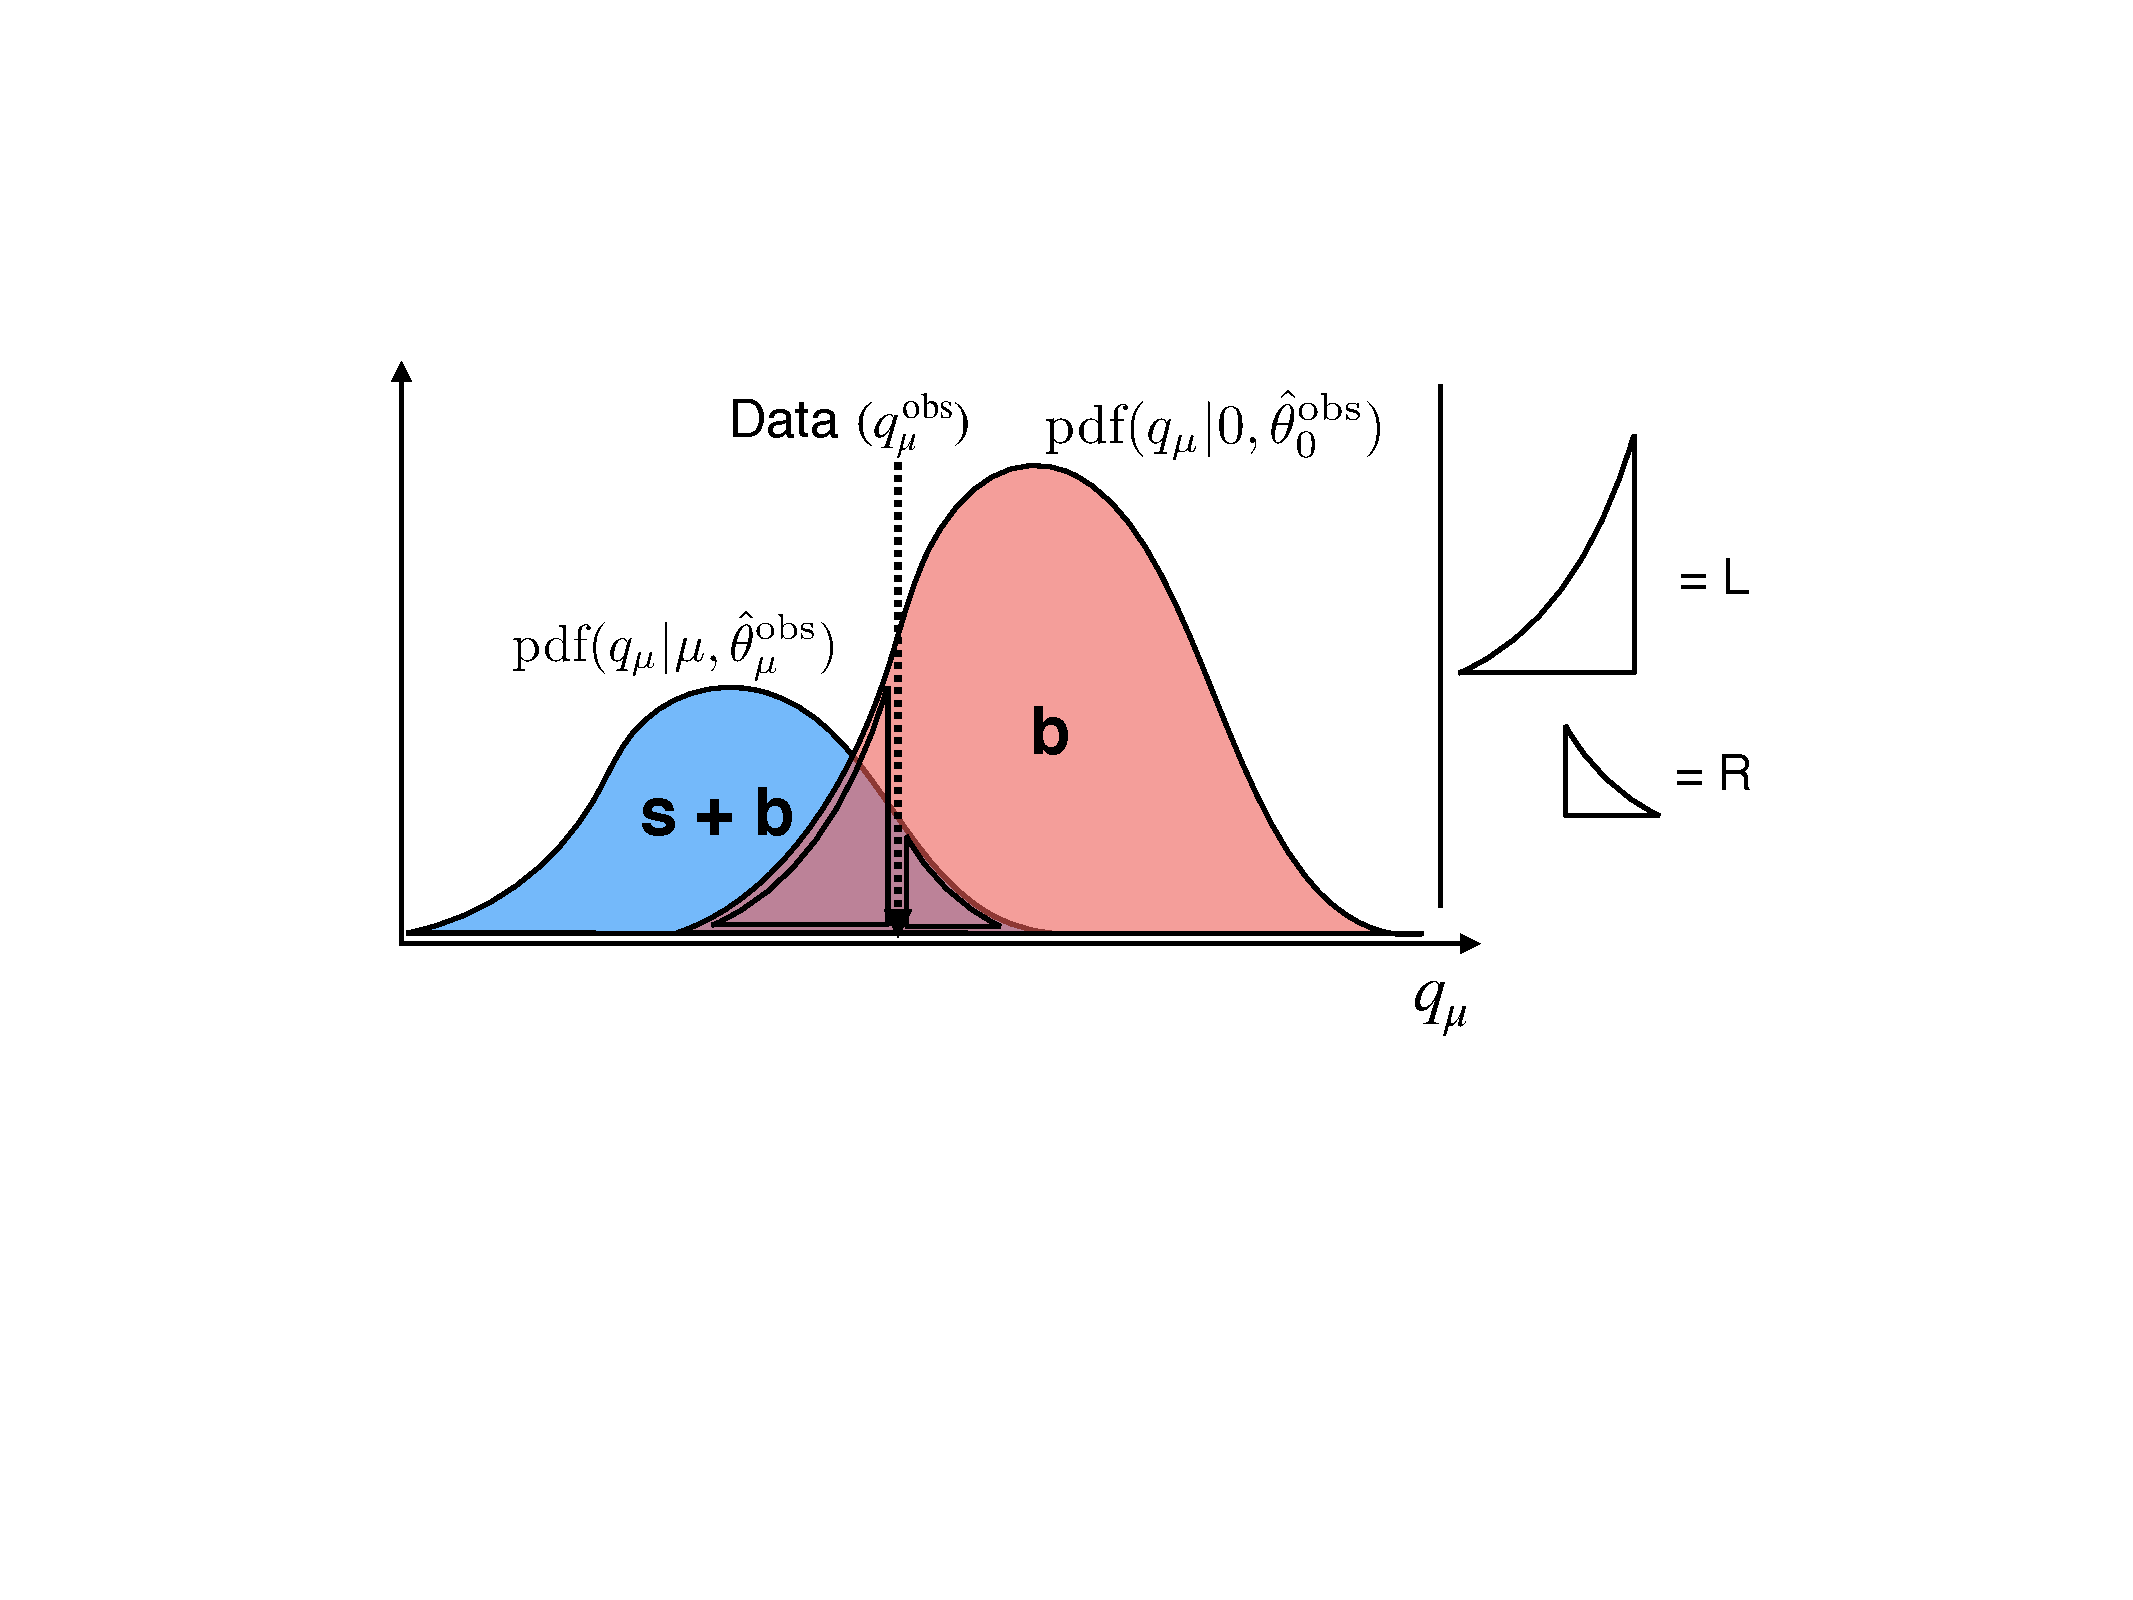
\includegraphics[width=0.85\linewidth]{figs/toy_statistics/ulschematic.pdf}
    \caption{
        Schematic diagram illustrating the \CLs method as described in the text.
    }
    \label{fig:ulschematic}
\end{figure}


\end{subsection}


\end{section}
